\subsection{Calculus Testing}\label{ssec:appendix-calculus-tests}
    Output of command \texttt{python src/calculus/tests.py}
    \small\verbatiminput{meta/calculus-tests.out}\normalsize

\subsection{Graph Visualisation Source Sample}\label{ssec:appendix-graph-source}
    Sample output of file \texttt{src/visualisation/graph.js}
    \small\verbatiminput{meta/graph-source.out}\normalsize

\subsection{Full Chain of Diagram Reduction}\label{ssec:appendix-diagram-reduction}
    Full reduction of the union of the examples in~\ref{sssec:diagram-reductions}
    \begin{figure}[H]
        \centering
        \begin{subfigure}{0.4\linewidth}
            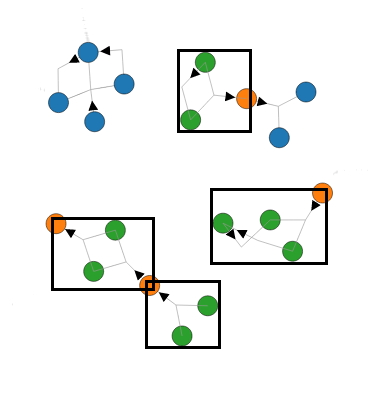
\includegraphics[width=\textwidth]{diagrams/all-diagrams.png}
        \end{subfigure}
        $\longrightarrow$
        \begin{subfigure}{0.4\linewidth}
            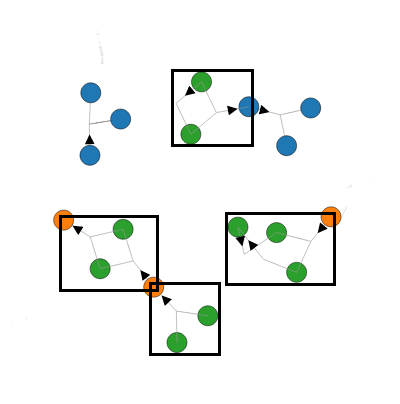
\includegraphics[width=\textwidth]{diagrams/all-diagrams-r1.png}
        \end{subfigure}
        $\longrightarrow$
    \end{figure}
    \begin{figure}[H]
        \centering
        \begin{subfigure}{0.4\linewidth}
            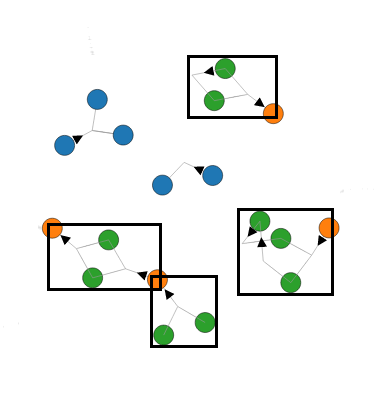
\includegraphics[width=\textwidth]{diagrams/all-diagrams-r2.png}
        \end{subfigure}
        $\longrightarrow$
        \begin{subfigure}{0.4\linewidth}
            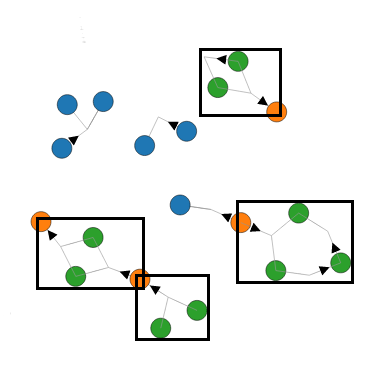
\includegraphics[width=\textwidth]{diagrams/all-diagrams-r3.png}
        \end{subfigure}
        $\longrightarrow$
    \end{figure}
    \begin{figure}[H]
        \centering
        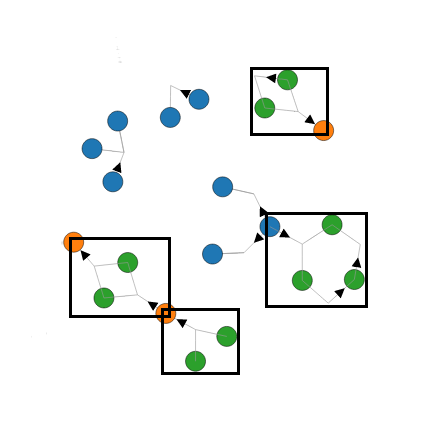
\includegraphics[width=0.4\textwidth]{diagrams/all-diagrams-r4.png}
    \end{figure}
